% \todo[inline]{unify lables of figures and tables}
%
% \bigskip
%
% \todo[inline]{\url{https://arxiv.org/pdf/cs/0108016.pdf}}
% \todo[inline]{\url{https://www.cl.cam.ac.uk/~pes20/weakmemory/cacm.pdf}}
% \todo[inline]{\url{https://mirrors.edge.kernel.org/pub/linux/kernel/people/paulmck/perfbook/perfbook-e2-rc9.pdf}}
% % CBMC
% \todo[inline]{\url{http://www.kroening.com/papers/tcad-sw-2008.pdf}}
% \todo[inline]{\url{http://www.kroening.com/papers/tacas2004.pdf}}
% \todo[inline]{\url{https://link.springer.com/content/pdf/10.1007/978-3-642-39799-8\_9.pdf}}
%
% \newpage

\section{Introduction}

%% sequential consistency:
%% \emph{``the result of any execution is the same as if the operations of all the processors were executed in some sequential order, and the operations of each individual processor appear in this sequence in the order specified by its program''}.

% \todo[inline]{need for software verification}\noindent

Correctness of computer systems is critical in today's information age and although software verification made considerable progress in the last decade, it is still an ongoing research topic.
Testing alone however is not sufficient to validate parallel programs
communicating via shared memory on modern multiprocessor hardware,
% running on current multiprocessor hardware
% and communicating via shared memory,
% running on modern shared memory multiprocessor hardware
as fatal race conditions can have extremely low probabilities of occurrence.
The situation becomes even worse due to counter-intuitive behaviour introduced by certain hardware optimizations.
Without further knowledge about the underlying architecture, inexperienced developers of
concurrent
low-level
systems code like lockless data structures, operating system kernels, synchronization
% libraries,
primitives,
% compilers and so on might assume that the order of access to memory is \emph{sequentially consistent}
% compilers and so on might assume a total order of access to memory for any possible interleaving, where each process is executed in program order.
compilers,
% etc.\
and so on
might assume
% that
% \emph{``the result of any execution is the same as if the operations of all the processors were executed in some sequential order for every possible interleaving and the operations of each individual processor appear in this sequence in the order specified by its program''}
% the result of any execution is the same as if the operations of all processors were executed in some sequential order and the operations of each individual processor appear program order.
\emph{sequential consistency} \cite{ref:Lamport79}.
Unfortunately, none of the major hardware architectures follows this rather restrictive \emph{memory ordering model} and allow
% memory access operations to be reordered
reordering of memory access operations
in various ways.
This opens the door for hard to find bugs caused by unexpected
% reorderings
behaviour
and
% needs to be prevented by
% requires careful use of the target architecture's memory barrier operations to ensure consistency.
requires a deep understanding of the target architecture's memory ordering habits,
% as well as
accompanied by careful use of \emph{memory barrier} operations to ensure consistency.
% referred to as \emph{sequential consistency} \cite{ref:Lamport79}.

% \bigskip

% For example, modern processors are equipped with a store buffer to speed up writes.

% \todo[inline]{counter-intuitive behaviour introduced by hardware optimizations}
% \todo[inline]{memory models}

% \bigskip

\tabulinesep=6pt
\noindent
\begin{table}[!hbt]
  \centering
  \begin{tabu}{|l|c|c|c|c|c|c|c|c|}
    \tabucline{2-}
    \multicolumn{1}{c|}{}
    & \rotatebox{90}{Alpha}
    & \rotatebox{90}{ARM}
    & \rotatebox{90}{Itanium}
    & \rotatebox{90}{MIPS}
    & \rotatebox{90}{POWER}
    & \rotatebox{90}{SPARC-TSO}
    & \rotatebox{90}{x86}
    & \rotatebox{90}{zSystems} \\
    \tabucline{2-}
    \firsthline
    Loads Reordered after Loads/Stores? & \cmark & \cmark & \cmark  & \cmark & \cmark & & & \\
    \hline
    Stores Reordered after Stores? & \cmark & \cmark & \cmark & \cmark & \cmark & & & \\
    \hline
    Stores Reordered after Loads? & \cmark & \cmark & \cmark & \cmark & \cmark & \cmark & \cmark & \cmark \\
    \hline
    Atomic Reordered with Loads/Stores? & \cmark & \cmark & & \cmark & \cmark & & & \\
    % \hline
    % Dependent Loads Reordered? & \cmark & & & & & & & \\
    % \hline
    % Dependent Stores Reordered & & & & & & & & \\
    \lasthline
  \end{tabu}
  % \caption{Summary of Memory Ordering}
  \caption{Memory Ordering on Different Architectures}
  \label{tbl:ordering}
\end{table}

% \subsection{Problem/Motivation}

% \todo[inline]{problems arising due to the unawareness of the specific architectures memory model}
% \todo[inline]{example for counter intuitive behaviour} \noindent

% Table \ref{tbl:ordering} shows that even the most restrictive architectures like the widely used x86

% The Intel-64 and AMD memory ordering models allow a load to be reordered with an earlier store to a different location, thus breaking sequential consistency.
% However, loads are not reordered with stores to the same location.
% Even though this is the only reordering allowed, it is sufficient for introducing counter intuitive behaviour, illustrated by the example given in Listing \ref{fig:intro:code}.

Table \ref{tbl:ordering} shows a rough overview of the memory ordering models used by different architectures.
Even the most restrictive -- like the x86 processors in our desktop computers -- allow loads to be reordered with an earlier store to a different location, thus breaking sequential consistency.
The reason for this particular reordering is a widely used optimization technique commonly referred to as \emph{store buffer}.

While caches improve subsequent repeated loads of a specific variable (after an initial cache miss),
% \todo[noline]{stolen from perfbook}
it is also necessary to accommodate frequent concurrent stores from multiple processors to a set of shared variables.
In cache-coherent systems, if the caches hold multiple copies of a given variable, all the copies of that variable must have the same value.
Each store will therefore invalidate all copies of the old value,
% resulting in even more cache misses
hence slowing down the computation % significantly.
\cite{ref:McKenney17}.

% \todo[inline]{reordering introduced by store buffers}

\begin{figure}[!h]
  \centering
  % styles
\tikzstyle{box} = [draw, text centered, rounded corners]
\tikzstyle{processor} = [box, fill=blue!10]
\tikzstyle{buffer} = [box, fill=red!10]
\tikzstyle{cache} = [box, fill=yellow!10]

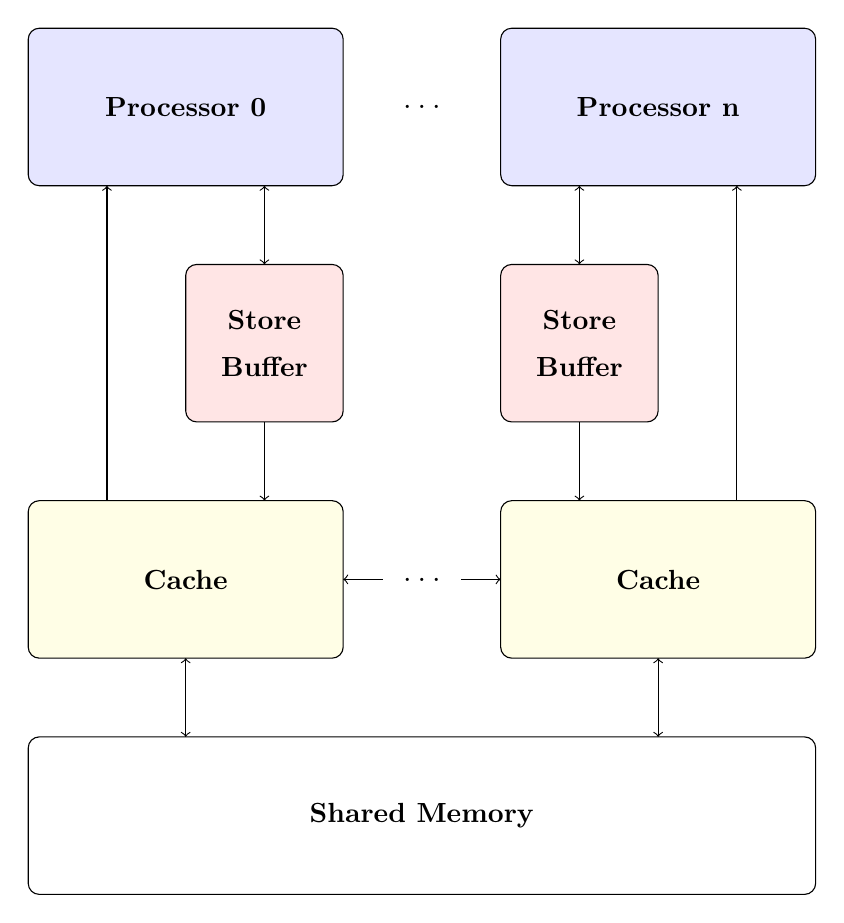
\begin{tikzpicture}

  % \draw[step=1cm,gray,very thin] (-5, 0) grid (5, -10);

  % processors
  \path [processor] (-5, 0) rectangle (-1, -2);
  \path (-3, -1) node (p-0) [] {\textbf{Processor 0}};

  \path [processor] (1, 0) rectangle (5, -2);
  \path (3, -1) node (p-n) [] {\textbf{Processor n}};

  % store buffers
  \path [buffer] (-3, -3) rectangle (-1, -5);
  \path (-2, -3.7) node (s-0) [] {\textbf{Store}};
  \path (-2, -4.3) node (b-0) [] {\textbf{Buffer}};

  \path [buffer] (1, -3) rectangle (3, -5);
  \path (2, -3.7) node (s-n) [] {\textbf{Store}};
  \path (2, -4.3) node (b-n) [] {\textbf{Buffer}};

  % caches
  \path [cache] (-5, -6) rectangle (-1, -8);
  \path (-3, -7) node (c-0) [] {\textbf{Cache}};

  \path [cache] (1, -6) rectangle (5, -8);
  \path (3, -7) node (c-n) [] {\textbf{Cache}};

  % heap
  \path [box] (-5, -9) rectangle (5, -11);
  \path (0, -10) node (heap) [] {\textbf{Shared Memory}};

  % arrows
  \path [draw, <-] (-4, -2) -- (-4, -6);  % cache -> processor 0
  \path [draw, <->] (-2, -2) -- (-2, -3); % sb <-> processor 0
  \path [draw, ->] (-2, -5) -- (-2, -6);  % sb -> cache
  \path [draw, <->] (-3, -8) -- (-3, -9); % cache <-> memory

  \path [draw, <-] (4, -2) -- (4, -6);    % cache -> processor n
  \path [draw, <->] (2, -2) -- (2, -3);   % sb -> processor n
  \path [draw, ->] (2, -5) -- (2, -6);    % sb -> cache
  \path [draw, <->] (3, -8) -- (3, -9);   % cache <-> memory

  \path [draw, <-] (-1, -7) -- (-0.5, -7);
  \path (0, -7) node (dots) [] {\large $\ldots$};
  \path [draw, ->] (0.5, -7) -- (1, -7);

  % dots
  \path (0, -1) node (dots) [] {\large $\ldots$};

\end{tikzpicture}

  \caption{System Architecture with Store Buffers}
  \label{fig:intro:store-buffer-architecture}
\end{figure}

To remedy this situation, modern processors come equipped with store buffers, as shown in Figure \ref{fig:intro:store-buffer-architecture}.
When a variable is stored, the new value is placed in the processor's store buffer, which can proceed immediately without having to wait for the store to do something about all the old values of that variable residing in other processors' caches.
% store forwarding
In order to guarantee that each processor at least sees its own operations in program order, it first examines its store buffer before consulting the cache when loading a variable in a process called \emph{store forwarding}.
% store buffer flushes
% flushes and memory barrier operations (explicit and implicit - OS issue a memory barrier before switching contexts)
% arbitrarily delaying visibility of the store to other processors.
% Each store buffer is allowed to voluntarily flush its contents back to memory, or may be forced to do so by certain instructions like memory barriers.
Since each store buffer is allowed to voluntarily flush its contents back to memory, the visibility of the particular stores to other processors might be arbitrarily delayed, leading to the aforementioned memory misordering
illustrated by the store buffer litmus test shown in Listing \ref{lst:intro:store-buffer-litmus}.
% If the processor is not forced to flush its contents back to memory, visibility of stores to other processors is arbitrarily delayed, leading to the aforementioned misordering.
% This leads to the aforementioned misordering, as the particular stores' visibility to other processor might be arbitrarily delayed.
% This simple optimization is sufficient for introducing the aforementioned misordering, as the particular stores' visibility to other processor might be arbitrarily delayed.

\begin{lstlisting}[style=c++, numbers=left, numberstyle=\footnotesize, numberblanklines=false, caption={Store Buffer Litmus Test}, label={lst:intro:store-buffer-litmus}]
#include <assert.h>
#include <pthread.h>

#define ACCESS(x) (*(volatile typeof(x) *) &(x))
#define READ(x) ({typeof(x) TMP = ACCESS(x); TMP;})
#define WRITE(x,v) ({ACCESS(x) = (v);})

static int w0 = 0;
static int w1 = 0;

static int r0 = 0;
static int r1 = 0;

static void * P0 (void * p)
{
  WRITE(w0, 1);
  r0 = READ(w1);
  return p;
}

static void * P1 (void * p)
{
  WRITE(w1, 1);
  r1 = READ(w0);
  return p;
}

int main ()
{
  pthread_t t[2];
  pthread_create (t + 0, 0, P0, 0);
  pthread_create (t + 1, 0, P1, 0);
  pthread_join (t[0], 0);
  pthread_join (t[1], 0);
  assert(r0 + r1);
  return 0;
}
\end{lstlisting}

% \todo[inline]{x86 permits $\texttt{r0 = 0} \land \texttt{r1 = 0}$}
One might assume that the assertion on line 35 never triggers, because any possible interleaving should guarantee that at least one \lstinline[style=c++]{WRITE} must have happened before a subsequent \lstinline[style=c++]{READ} by the other thread in this symmetric example.
This intuition however breaks down with the addition of store buffers.
Consider the interleavings depicted in Figure \ref{fig:intro:store-buffer-litmus-interleaving}.
\begin{figure}[!h]
  \centering
  \begin{tikzpicture}

  \path (0, 0) node (init) [] {$w_0 = w_1 = 0$};
  \path (0, -6) node (join) [] {$r_0 + r_1 = 0$};

  \path (-3, -2) node (w0) [red] {$w_0 = 1$};
  \path [->] (init) edge node [above] {$t_0$} (w0);
  \path (-3, -4) node (r0) [] {$r_0 = w_1 = 0$};
  \path [->] (w0) edge node [left] {$t_0$} (r0);
  \path [->] (r0) edge node [below] {$t_0$} (join);

  \path (3, -2) node (w1) [red] {$w_1 = 1$};
  \path [->] (init) edge node [above] {$t_1$} (w1);
  \path (3, -4) node (r1) [] {$r_1 = w_0 = 0$};
  \path [->] (w1) edge node [right] {$t_1$} (r1);
  \path [->] (r1) edge node [below] {$t_1$} (join);

  \path (0, -2) node (buffered) [red] {buffered};
  \path [draw, dotted, red, <-] (w0) -- (buffered);
  \path [draw, dotted, red, ->] (buffered) -- (w1);

  \path [draw, dotted, ->] (init) -- (r0);
  \path [draw, dotted, ->] (init) -- (r1);

  % forwarding arrows

  % \path [draw, dotted, green, ->] (init) edge node [near end, left] {\cmark} (r0);
  % \path [draw, dotted, green, ->] (init) edge node [near end, right] {$\;$\cmark} (r1);

  % \path [dotted, red, ->] (w1) edge node [near end, below] {\xmark} (r0);
  % \path [dotted, red, ->] (w0) edge node [near end, below] {\xmark} (r1);

  % \path (0, -1.2) node (mem) [green] {memory};
  % \path (0, -3.6) node (sb) [red] {buffered};

  % alternative figure

  % \path (0, -10) node (Xinit) [draw, rounded corners, text centered, inner sep=0pt] {
    % \begin{tabu}{c}
      % \footnotesize memory \\
      % $w_0 = w_1 = r_0 = r_1 = 0$ \\
    % \end{tabu}
  % };
%
  % \path (-3, -13) node (Xw0) [draw, rounded corners, text centered, inner sep=0pt] {
    % \begin{tabu}{c}
      % \textbf{thread 0} \\
      % \hline
      % \footnotesize memory \\
      % $w_1 = r_0 = r_1 = 0$ \\
      % % \tabucline[on 1pt off 2pt]{-}
      % \hline
      % \footnotesize store buffer \\
      % % \tabucline[on 1pt off 2pt]{-}
      % $w_0 = 1$
    % \end{tabu}
  % };
%
  % \path (-3, -17) node (Xr0) [draw, rounded corners, text centered, inner sep=0pt] {
    % \begin{tabu}{c}
      % \textbf{thread 0} \\
      % \hline
      % \footnotesize memory \\
      % $w_1 = r_0 = r_1 = 0$ \\
      % % \tabucline[on 1pt off 2pt]{-}
      % \hline
      % \footnotesize store buffer \\
      % % \tabucline[on 1pt off 2pt]{-}
      % $w_0 = 1\;$
    % \end{tabu}
  % };
%
  % \path [->] (Xinit) edge node [left] {$w_0 = 1$} (Xw0);
  % \path [->] (Xw0) edge node [left] {$r_0 = w_1$} (Xr0);
\end{tikzpicture}

  \caption{Store Buffer Litmus Test Interleavings}
  \label{fig:intro:store-buffer-litmus-interleaving}
\end{figure}
After initializing the shared variables with zero, %($w_0 = w_1 = 0$)
% both
writes to $w_0$ and $w_1$ will be placed into the respective processor's store buffer.
If neither of the store buffers has been flushed prior to the subsequent reads $r_0 = w_1$ and $r_1 = w_0$, both processors must resort to the variable's initial value in their caches,
% which still contains the initial value,
hence triggering the assertion.
% Since it still contains their initial value,
% the threads will erroneously load zero,
% hence triggering the assertion.
% \todo[inline]{\texttt{experiments/demo/run.sh}: 177169 out of 1000000 failed = $\sim 17.7$ \% ($\sim 12$ min)}
% \todo[inline]{only 82 out of 1000000 returned the perfectly legal outcome of 2}
This willingness to reorder can be validated by running the store buffer litmus test given in Listing \ref{lst:intro:store-buffer-litmus}.
On our Intel i7-3770K this counter-intuitive reordering happened 177169 out of 1000000 test runs, while the perfectly legal outcome of $r_0 + r_1 = 2$ on the other hand only occurred 82 times.

% \todo[inline]{lack of concrete, formal specifications what programmers can rely on}
Programmers must therefore make careful use of memory barriers,
forcing the store buffer to be flushed back to memory after writing to a shared variable whenever necessary.
Unfortunately, many hardware vendors don't supply concrete formal specifications programmers can rely on.
For example, the memory ordering models of Intel's \cite{ref:Intel} as well as AMD's \cite{ref:AMD} x86 implementations are specified in an informal prose together with a set of litmus tests, having the potential for leading to widespread confusion.

% \subsection{Toolchain}

% \bigskip
\newpage
% \noindent

In this thesis we tried to address this issue by
% exploring encodings of an abstract machine model including memory ordering.
means of \emph{bounded model checking} \cite{ref:BMC}
based on the architectural view of a simple virtual machine model using store buffers,
reassambling the memory ordering habits of
the industry's leading
% current
x86 implementations.
% on the basis of a simple virtual machine model including store buffers.
% and explored encodings of an abstract machine model including memory ordering.
In order to evaluate our approach we developed
ConcuBinE\footnote{\url{https://github.com/phlo/concubine}} (short for \textbf{Concu}rrent \textbf{Bin}ary \textbf{E}valuator),
a tool for simulating and
% verifying
automated reasoning about
random memory access sequences by
concurrent programs.
% on a virtual machine using store buffers,
% dubbed ConcuBinE\footnote{\url{https://github.com/phlo/concubine}} (\textbf{Concu}rrent \textbf{Bin}ary \textbf{E}valuator).
It offers three modes of execution:
\begin{itemize}
  \item \texttt{simulate}:
    simulates the execution of given programs and returns the corresponding execution trace in an easy to read format.
  \item \texttt{solve}:
    automatically generates an encoding of given programs for a specific upper bound and evaluates the resulting bounded model checking problem with the help of state-of-the-art SMT solvers.
    If the problem is satisfiable, the corresponding execution trace (model) will be returned.
  \item \texttt{replay}:
    % used to validate a given trace via simulation.
    reevaluates a given trace via simulation.
    Used to validate the traces found by the \texttt{solve} mode.
\end{itemize}
Figure \ref{fig:intro:toolchain} shows a basic overview of its usage,
where red nodes symbolize in and output files,
% blue nodes the components according to the mode it is used
blue nodes the mode of opration
and yellow nodes external software (SMT solvers).

% In this thesis we developed a toolchain for simulating and bounded model checking of random memory access sequences by concurrent programs.

% \bigskip
% In this thesis we tried to address this issue by developing a toolchain for simulating and
% automated reasoning about
% % random memory access sequences of
% concurrent programs by means of \emph{bounded model checking} \cite{ref:BMC}.
% Instead of real hardware, it is based on the architectural view of a simple virtual machine model abstracting caches but

% \bigskip

% \todo[inline]{address the problem by the means of bounded model checking}
% \todo[inline]{ConcuBinE
% /ˈkɒŋ.kjə.baɪn/
% \textbf{Concu}rrent \textbf{Bin}ary \textbf{E}valuator - a toolchain for simulating and bounded model checking of random memory access sequences by concurrent programs on a simple virtual machine using store buffers.}
% \todo[inline]{components structured according to the mode they are used}

\begin{figure}[h]
  \centering
  % styles
\tikzstyle{module} = [draw, fill=blue!10, text centered, rounded corners, minimum height=1cm, minimum width=2.5cm]
\tikzstyle{file} = [module, fill=red!10]
\tikzstyle{external} = [module, fill=yellow!10]

\begin{tikzpicture}[auto]

  \node [file] (program) {program};

  \node [module] (simulate) [above right=0cm and 1cm of program] {\texttt{simulate}};
  \path [draw, ->] (program.east) -- ++(0.5, 0) |- (simulate);

  \node [module] (solve) [below right=0cm and 1cm of program] {\texttt{solve}};
  \path [draw, ->] (program.east) -- ++(0.5, 0) |- (solve);

  \node [external] (solver) [below= of solve] {SMT solver};
  \path [draw, ->, transform canvas={xshift=-0.5cm}] (solve) -- (solver);
  \path [draw, <-, transform canvas={xshift=0.5cm}] (solve) -- (solver);

  \node [file] (trace) [below right=0cm and 1cm of simulate] {trace};
  \path [draw, ->] (simulate.east) -- ++(0.5, 0) |- (trace);
  \path [draw, ->] (solve.east) -- ++(0.5, 0) |- (trace);

  \node [module, dashed] (replay) [right= of trace] {\texttt{replay}} edge [<-, dashed] (trace);
  \path [draw, dashed, ->] (replay) -- (replay.north |- simulate) -| (trace.north);

\end{tikzpicture}

  \caption{ConcuBinE's Various Modes of Operation}
  \label{fig:intro:toolchain}
\end{figure}
